\documentclass[11pt]{article}
\usepackage[margin=1.0in]{geometry}
\usepackage{mathtools}
\usepackage{graphicx}
\usepackage{float}
\usepackage[font=small]{caption}
\usepackage{color}
\usepackage{fancyhdr}
%\usepackage{soul} %for striking out text
%\usepackage{arydshln} % for dotted line on truth table
\usepackage{tikz} % graphics stuff
\usepackage{caption}
\usepackage{gensymb}
\usepackage{booktabs}
\usepackage{listings}
\usepackage{fancyvrb}
%\usepackage{subcaption} % used to horizontally tile figures
%\usepackage{listings}
\pagestyle{fancy}
\fancyhead{}
\fancyfoot{}
\fancyfoot[R]{\thepage}

\definecolor{mygreen}{rgb}{0,0.6,0}
\definecolor{mygray}{rgb}{0.5,0.5,0.5}
\definecolor{mymauve}{rgb}{0.58,0,0.82}

\lstset{ 
	backgroundcolor=\color{white},   % choose the background color; you must add \usepackage{color} or \usepackage{xcolor}; should come as last argument
	basicstyle=\footnotesize,        % the size of the fonts that are used for the code
	breakatwhitespace=false,         % sets if automatic breaks should only happen at whitespace
	breaklines=true,                 % sets automatic line breaking
	captionpos=t,                    % sets the caption-position to bottom
	commentstyle=\color{mygreen},    % comment style
	deletekeywords={},               % if you want to delete keywords from the given language
	escapeinside={\%*}{*)},          % if you want to add LaTeX within your code
	extendedchars=false,             % lets you use non-ASCII characters; for 8-bits encodings only, does not work with UTF-8
	firstnumber=0,                   % start line enumeration with line 1000
	frame=single,                    % adds a frame around the code
	keepspaces=true,                 % keeps spaces in text, useful for keeping indentation of code (possibly needs columns=flexible)
	keywordstyle=\color{blue},       % keyword style
	language=VHDL,                   % the language of the code
	morekeywords={},                 % if you want to add more keywords to the set
	numbers=left,                    % where to put the line-numbers; possible values are (none, left, right)
	numbersep=5pt,                   % how far the line-numbers are from the code
	numberstyle=\tiny\color{mygray}, % the style that is used for the line-numbers
	rulecolor=\color{black},         % if not set, the frame-color may be changed on line-breaks within not-black text (e.g. comments (green here))
	showspaces=false,                % show spaces everywhere adding particular underscores; it overrides 'showstringspaces'
	showstringspaces=false,          % underline spaces within strings only
	showtabs=false,                  % show tabs within strings adding particular underscores
	stepnumber=5,                    % the step between two line-numbers. If it's 1, each line will be numbered
	stringstyle=\color{mymauve},     % string literal style
	tabsize=4, 	                     % sets default tabsize to 2 spaces
	title=\lstname                   % show the filename of files included with \lstinputlisting; also try caption instead of title
}

\begin{document}

%
% cover page
%

\vspace*{2 cm}

\begin{center}
\bf{CMPE-630 Digital IC Design\\
    Laboratory Exercise 7\\
\vspace{0.25 cm}
Autolayout Design Techniques (HDL-Layout)
}
\end{center}

\vspace{6 cm}

\begin{flushright}
Brandon Key and Chris Guarini\\
Performed: 9 Dec 2019\\
Submitted: 9 Dec 2019\\
\vspace{0.5 cm}
Instructor: Dr. Amlan Ganguly\\
TAs: Abhishek Vashist\\
Andrew Fountain\\
Piers Kwan\\
\vspace{0.5 cm}
\end{flushright}

\vspace{3 cm}
\indent By submitting this report, you attest that you neither have given nor have received any assistance (including writing, collecting data, plotting figures, tables or graphs, or using previous student reports as a reference), and you further acknowledge that giving or receiving such assistance will result in a failing grade for this course.

\vspace{1 cm}
Your Signature:   \rule{13cm}{.1pt}


\tableofcontents
\newpage

\section{Abstract}

	Integrated Circuit Design is a costly and complex endeavor. Fortunately, automatic tools speed up the process and allow designs that are not possible to create manually. This exercise implemented a 1-Bit ALU and a 16-Bit ALU using autolayout. The autolayout tools generated very reasonable circuits. The 1-Bit ALU has an input frequency of 380.92MHz and a throughput frequency of 553.4MHz, while the 16-bit ALU has an input frequency of 461.02MHz and a throughput frequency of 110.2MHz. The area used by the ALUs was also reasonable with the 1-bit ALU taking up 647.89$\mu m^2$ and the 16-bit ALU occupying 9792.5$\mu m^2$.
	

\section{Design Methodology and Theory}

	A cornerstone of IC design is the ability to create large, complex designs from smaller more manageable parts. The project outlined in this exercise calls for the design, testing and layout of a multiply and accumulate (MAC) unit, which takes two 16-bit inputs, multiplies them together, adds them to the value stored in a register, and then stores that output back into the register. The final component should contain a built in self test (BIST) that verifies the functionality of the MAC.
	
	The MAC is composed of a carry-save multiplier, ripple carry full-adder, and parallel register. The BIST is implemented through the use of an LFSR for the inputs, an MISR for the output, and a test controller which controls the timing and sets the test passed and test complete outputs. A full diagram of the MAC with BIST can be seen below in \textit{Figure 1}.
	
	\begin{figure}
		\centering
		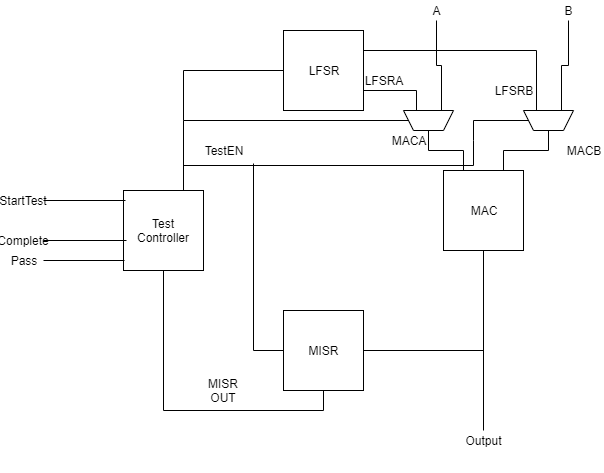
\includegraphics[width=0.7\linewidth]{Report/Pictures/Full-Project-Block}
		\caption{\textbf{Figure 1: } High Level Block Diagram of the MAC with BIST.}
		\label{fig:full-project-block}
	\end{figure}
	

	\subsection{Functional Simulation}
	

		The ALUs in this exercise had a simple 2 bit op-code which can be seen in Table \ref{tab:OpCodes}.
	
		\begin{table}[H]
			\centering
			\caption{ALU Operations}
			\label{tab:OpCodes}
			\begin{tabular}{|ccc|}
				\hline
				\textbf{OpCode} & \textbf{Operation} & \textbf{Operands} \\
				\hline
				00              & AND                & A AND B           \\
				01              & OR                 & A OR B            \\
				10              & ADD                & A + B             \\
				11              & SUB                & A - B   \\   
				\hline       
			\end{tabular}
		\end{table}
	
		\subsubsection{1 Bit ALU}
		
			The 1 Bit ALU designed in this exercise was created from behavioral VHDL (see Listing \ref{lst:ALU-1Bit}). A Questa Sim simulation was performed to test the functionality of the 1 bit ALU. The test bench can be seen in Listing \ref{lst:ALU-1Bit-tb}. The test bench went through every op-code and every input. The resulting waveforms can be seen in Figure \ref{fig:alu1bit-functional-sim-}.
		
			\begin{figure}[H]
				\centering
				\includegraphics[width=1\linewidth]{"Pictures/ALU_1Bit Functional Sim "}
				\caption{Functional Simulation of 1-bit ALU}
				\label{fig:alu1bit-functional-sim-}
			\end{figure}
		
			The 1 Bit ALU functioned properly.
		
		\subsubsection{16 Bit ALU}
		
			The 16-bit ALU was created structurally with generically large structures. The VHDL that describes the ALU can be seen in Listing \ref{lst:ALU-16Bit}. While the 1-bit ALU could have a full test bench that tested every input, the 16-bit ALU was far too large to do the same. Instead, a few test cases were selected to test each function of the ALU. Each component in the ALU was previously tested, so the main goal was to test the setup of the ALU itself. The testbanch code can be seen in Listing \ref{lst:ALU-16Bit-tb}. The AND functionality was tested first and captured in Figure \ref{fig:16-bit-alu-and}.
		
			\begin{figure}[H]
				\centering
				\includegraphics[width=0.7\linewidth]{"Pictures/16 Bit ALU AND"}
				\caption{Functional Simulation of 16-bit ALU: AND}
				\label{fig:16-bit-alu-and}
			\end{figure}
		
			Once the and functionality was verified, the OR functionality was tested and recorded in Figure \ref{fig:16-bit-alu-or}.
		
			\begin{figure}[H]
				\centering
				\includegraphics[width=0.7\linewidth]{"Pictures/16 Bit ALU OR"}
				\caption{Functional Simulation of 16-bit ALU: OR}
				\label{fig:16-bit-alu-or}
			\end{figure}
			
			The OR operation worked properly, so addition was tested and recorded in Figure \ref{fig:16-bit-alu-add}.
			
			\begin{figure}[H]
				\centering
				\includegraphics[width=0.7\linewidth]{"Pictures/16 Bit ALU Add"}
				\caption{Functional Simulation of 16-bit ALU: Addition}
				\label{fig:16-bit-alu-add}
			\end{figure}
		
			More test cases were added to addition so that the carry bit was tickled. This simulation was recorded in Figure \ref{fig:16-bit-alu-add-carry}.
			
			\begin{figure}[H]
				\centering
				\includegraphics[width=0.7\linewidth]{"Pictures/16 Bit ALU Add Carry"}
				\caption{Functional Simulation of 16-bit ALU: Addition with carry}
				\label{fig:16-bit-alu-add-carry}
			\end{figure}
			
			Add functionality worked, so the same was done with the subtraction operation. Figure \ref{fig:16-bit-alu-sub-pos} shows subtraction with a positive result.
			
			\begin{figure}[H]
				\centering
				\includegraphics[width=0.7\linewidth]{"Pictures/16 Bit Alu Sub Pos"}
				\caption{Functional Simulation of 16-bit ALU: Subtraction}
				\label{fig:16-bit-alu-sub-pos}
			\end{figure}
		
			Figure \ref{fig:16-bit-alu-sub-neg} show subtraction with a negative result.
			
			\begin{figure}[H]
				\centering
				\includegraphics[width=0.7\linewidth]{"Pictures/16 Bit ALU Sub Neg"}
				\caption{Functional Simulation of 16-bit ALU: Subtraction with negative result}
				\label{fig:16-bit-alu-sub-neg}
			\end{figure}
		
			Subtraction with the 16-bit ALU was correct, thus rounding out the functional testing of the design. Next, a schematic could be created.

	\subsection{Schematic}
	
		Schematics were generated by Pyxis Schematic Editor. The tool generated a nearly complete schematic(s), but the component layout needed adjustment as some inverters were overlapping. 

		\subsubsection{1-Bit ALU}	
		
			The 1-bit ALU schematic spanned one page and can be seen in Figure \ref{fig:alu-1bit-schematic}. 
			
			\begin{figure}[H]
				\centering
				\includegraphics[width=0.4\linewidth]{"Pictures/ALU-1Bit Schematic"}
				\caption{1 Bit ALU Schematic}
				\label{fig:alu-1bit-schematic}
			\end{figure}
		
			The 1-bit ALU is rather simple.		

		\subsubsection{n-Bit ALU}
		
			Pyxis created 3 schematic sheets to satisfy the 16-bit ALU. This likely due to the structural nature of the ALU. The schematic can be seen in Figure \ref{fig:alu-16bit-schematic-1} through Figure \ref{fig:alu-16bit-schematic-3}.
			
			
			\begin{figure}[H]
				\centering
				\includegraphics[width=0.3\linewidth]{"Pictures/ALU-16Bit Schematic 1"}
				\caption{16 Bit ALU Schematic Page 1}
				\label{fig:alu-16bit-schematic-1}
			\end{figure}
		
			\begin{figure}[H]
				\centering
				\includegraphics[width=0.2\linewidth]{"Pictures/ALU-16Bit Schematic 2"}
				\caption{16 Bit ALU Schematic Page 2}
				\label{fig:alu-16bit-schematic-2}
			\end{figure}
		
			\begin{figure}[H]
				\centering
				\includegraphics[width=0.4\linewidth]{"Pictures/ALU-16Bit Schematic 3"}
				\caption{16 Bit ALU Schematic Page 3}
				\label{fig:alu-16bit-schematic-3}
			\end{figure}

			The 16-bit ALU is dramatically more complex than the single bit ALU.

\section{Results and Analysis}
		
	The ALUs in this exercise had a layout created for them. Then the layout was compared to the schematic via a LVS check. Then timing data was extracted with a PEX extraction. A simulation was run off of the PEX results. Finally, static and dynamic power was measured from the circuit.
		
	\subsection{Layout}
		
		Pyxis was used to instantiate components from the schematic. Ports were added to the design before a floor plan was generated. To aid in the routing procedure, the area ratio was decreased from 1 to 0.7. Decreasing this area gives room between the cells to route wires. Standard cells were created with default settings. Power routing was run to ease the burden on auto routing and also to clean up the layout. Auto routing settings were adjusted to not route with poly silicon as this tends to cause stray gates. Additionally, the following settings were applied to aid in auto routing:
		\begin{itemize}
			\item Varying levels of routing completion time
			\item Slight preference for jogs over via to fill the area.
			\item Rip
			\item Under rip options: 
			\subitem Rips Most Aggressive
			\subitem Automatic Rip Passes
			\subitem Reroute
			\item Under Advanced:
			\subitem Allow all directions for stubs
			\subitem Via Options $>$ Use via generator
		\end{itemize}
	
		\subsubsection{1 Bit ALU}
		
			The one bit ALU can be seen in Figure \ref{fig:alu-1bit-layout}.
		
			\begin{figure}[H]
				\centering
				\includegraphics[width=0.7\linewidth]{"Pictures/ALU 1-Bit Layout"}
				\caption{1 Bit ALU Layout}
				\label{fig:alu-1bit-layout}
			\end{figure}
			
			The 1-bit ALU was 24.045$\mu$m wide and 26.945$\mu$m tall, for a total area of 647.893$\mu m^2$.
	
		\subsubsection{16 Bit ALU}
		
			The one bit ALU can be seen in Figure \ref{fig:alu-16bit-layout}.
		
			\begin{figure}[H]
				\centering
				\includegraphics[width=0.7\linewidth]{"Pictures/ALU 16-Bit Layout"}
				\caption{16 Bit ALU Layout}
				\label{fig:alu-16bit-layout}
			\end{figure}
		
			The 1-bit ALU was 94.005$\mu$m wide and 104.170$\mu$m tall, for a total area of 9792.5$\mu m^2$.

	
	\subsection{Timing}
	
		A SPICE file was written for each ALU, which was based off of the PEX extraction netlist. Eldo was used to run the simulation and ezwave was used to view the waveform and measure rise time, fall time, and propagation delay.
		
		The simulation was run for worst case conditions which are laid out in Figure \ref{fig:simulation-parameters}. 
		
		\begin{figure}[H]
			\centering
			\includegraphics[width=0.4\linewidth]{"Pictures/Simulation Parameters"}
			\caption{Simulation Parameters}
			\label{fig:simulation-parameters}
		\end{figure}
		
		
		The maximum input and throughput frequencies were calculated from the measured timing values according to Equation \ref{eqn:Finputmax} and Equation \ref{eqn:Fthroughputmax} respectively. 
		
		\begin{equation}\label{eqn:Finputmax}
		F_{input,max} = \frac{1}{t_{rise}+t_{fall}}
		\end{equation}
		\begin{center}
			Equation \ref{eqn:Finputmax}: Max Input Frequency
		\end{center}
		
		\begin{equation}\label{eqn:Fthroughputmax}
		F_{throughput,max} = \frac{1}{T_{P,HL}+T_{P,LH}}
		\end{equation}
		\begin{center}
			Equation \ref{eqn:Fthroughputmax}: Max Throughput Frequency
		\end{center}
	
		\subsubsection{1 Bit ALU}
			It was found that subtraction was by far the slowest operation, with the timing difference visible in the waveforms.  The SPICE file used to extract timing can be found in Listing \ref{lst:ALU-1-Bit-Spice}. The waveform and measurements can be seen in Figure \ref{fig:alu1bit-timing}.
		
			\begin{figure}[H]
				\centering
				\includegraphics[width=1\linewidth]{"Pictures/ALU_1Bit Timing"}
				\caption{1 Bit ALU Worst Case Timing Simulation}
				\label{fig:alu1bit-timing}
			\end{figure}
		
			The rise time was recorded in Table \ref{tab:ALU-1-Bit-Risetime}.
			
			\begin{table}[H]
				\centering
				\caption{1-Bit ALU Worst Case Rise Time}
				\label{tab:ALU-1-Bit-Risetime}
				\begin{tabular}{|cclcr|}
					\hline
					\textbf{Output} & \textbf{Rise Time (ps)} & \textbf{A} & \textbf{B} & \textbf{Operation} \\
					Y               & 1167.5                  & 1          & 0          & SUB                \\
					Carry           & 1557.1                  & 0          & 1          & SUB                \\
					         \hline
				\end{tabular}
			\end{table}
		
			The fall time was recorded in Table \ref{tab:ALU-1-Bit-Falltime}.
		
			\begin{table}[H]
				\centering
				\caption{1-Bit ALU Worst Case Fall Time}
				\label{tab:ALU-1-Bit-Falltime}
				\begin{tabular}{|cclcr|}
					\hline
					\textbf{Output} & \textbf{Fall Time (ps)} & \textbf{A} & \textbf{B} & \textbf{Operation} \\
					Y               & 1001.3                  & 1          & 1          & SUB                \\
					Carry           & 1068.1                  & 1          & 1          & SUB                \\
					\hline
				\end{tabular}
			\end{table}
		
			The propagation delay from high output to low output was recorded in Table \ref{tab:ALU-1-Bit-Tpd-HL}.
		
			\begin{table}[H]
				\centering
				\caption{1-Bit ALU Worst Case Propagation Time High to Low}
				\label{tab:ALU-1-Bit-Tpd-HL}
				\begin{tabular}{|cclcr|}
					\hline
					\textbf{Output} & \textbf{Tp,HL (ps)} & \textbf{A} & \textbf{B} & \textbf{Operation} \\
					Y               & 701.8                   & 1          & 1          & SUB                \\
					Carry           & 810.3                   & 1          & 1          & SUB                \\
					\hline
				\end{tabular}
			\end{table}
		
			The propagation delay from low output to high output was recorded in Table \ref{tab:ALU-1-Bit-Tpd-LH}.
		
			\begin{table}[H]
				\centering
				\caption{1-Bit ALU Worst Case Propagation Time Low to High}
				\label{tab:ALU-1-Bit-Tpd-LH}
				\begin{tabular}{|cclcr|}
					\hline
					\textbf{Output} & \textbf{Tp,LH (ps)} & \textbf{A} & \textbf{B} & \textbf{Operation} \\
					Y               & 686.1                   & 1          & 0          & SUB                \\
					Carry           & 996.7                   & 0          & 1          & SUB                \\
					\hline
				\end{tabular}
			\end{table}
		
			The frequency response was calculated and recorded in Table \ref{tab:ALU-1-Bit-Freq}.
		
			\begin{table}[H]
				\centering
				\caption{1-Bit ALU Calculated Max Frequency}
				\label{tab:ALU-1-Bit-Freq}
				\begin{tabular}{|ccc|}
					\hline
					\textbf{Output} & \textbf{Finput,max (MHz)} & \textbf{Fthroughput,max (MHz)} \\
					\hline
					Y               & 461.08                    & 720.51                         \\
					Carry           & 380.92                    & 553.40                         \\
					\hline
				\end{tabular}
			\end{table}
		
		\subsubsection{16 Bit ALU}
		
			The first SPICE file for the 16-bit ALU did not properly force the inputs, resulting in the waveform shown in Figure \ref{fig:terrible-simulation}.
		
			\begin{figure}[H]
				\centering
				\includegraphics[width=0.7\linewidth]{"Pictures/Terrible Simulation"}
				\caption{Simulation with Incorrect Forces}
				\label{fig:terrible-simulation}
			\end{figure}
			
			Listing \ref{lst:ALU-16-Bit-Spice} shows final the SPICE file used to simulate the 16-Bit ALU.  The waveform with timing measurement can be seen in Figure \ref{fig:alu-16-bit-full-timing}.
		
			\begin{figure}[H]
				\centering
				\includegraphics[width=1\linewidth]{"Pictures/ALU 16-Bit Full Timing"}
				\caption{16-Bit ALU Timing Waveforms}
				\label{fig:alu-16-bit-full-timing}
			\end{figure}
			
			The timing measurements were recorded in Table \ref{tab:ALU-16-Bit-Risetime} through Table \ref{tab:ALU-16-Bit-Tpd-LH}.
		
			\begin{table}[H]
				\centering
				\caption{16-Bit ALU Worst Case Rise Time}
				\label{tab:ALU-16-Bit-Risetime}
				\begin{tabular}{|cclcrcr|}
					\hline
					\multicolumn{2}{|c}{\textbf{Input}} & \textbf{Output} & \multicolumn{4}{c|}{\textbf{Rise Time (ps)}} \\
					\textbf{A} & \textbf{B} & \textbf{Y} & \textbf{Op} & \textbf{Y} & \textbf{Op} & \textbf{CB} \\
					\hline
					0x0000 & 0x0000 & Y{[}15{]} & 11 & 938.0 & 11 & 1033.8 \\
					0xFFFF & 0xFFFF & Y{[}15{]} & 11 & 938.0 & 01 & 1124.5 \\
					0xFFFF & 0x0001 & Y{[}15{]} & 11 & 982.2 & 11 & 1044.6 \\
					0x0001 & 0xFFFF & Y{[}15{]} & 01 & 904.63 & 00 & 1044.6 \\
					0x0000 & 0x0001 & Y{[}0{]} & 00 & 1085.2 & 01 & 986.9 \\
					0xABCD & 0x89EF & Y{[}15{]} & 01 & 917.9 & 11 & 951.8 \\
					\hline
				\end{tabular}
			\end{table}
		
		
			\begin{table}[H]
				\centering
				\caption{16-Bit ALU Worst Case Fall Time}
				\label{tab:ALU-16-Bit-Falltime}
				\begin{tabular}{|cclcrcr|}
					\hline
					\multicolumn{2}{|c}{\textbf{Input}} & \textbf{Output} & \multicolumn{4}{c|}{\textbf{Fall Time (ps)}} \\
					\textbf{A} & \textbf{B} & \textbf{Y} & \textbf{Op} & \textbf{Y} & \textbf{Op} & \textbf{CB} \\
					\hline
					0x0000 & 0x0000 & Y{[}15{]} & 01 & 1100.3 & 01 & 1027.1 \\
					0xFFFF & 0xFFFF & Y{[}15{]} & 10 & 1067.0 & 10 & 1033.8 \\
					0xFFFF & 0x0001 & Y{[}15{]} & 11 & 830.6 & 01 & 1124.5 \\
					0x0001 & 0xFFFF & Y{[}15{]} & 10 & 1161.7 & 11 & 951.8 \\
					0x0000 & 0x0001 & Y{[}0{]} & 00 & 996.8 & 10 & 1005.9 \\
					0xABCD & 0x89EF & Y{[}15{]} & 01 & 855.5 & 01 & 969.5 \\
					\hline
				\end{tabular}
			\end{table}
		
		
			\begin{table}[H]
				\centering
				\caption{16-Bit ALU Worst Case Propagation Time High to Low}
				\label{tab:ALU-16-Bit-Tpd-HL}
				\begin{tabular}{|cclcrcr|}
					\hline
					\multicolumn{2}{|c}{\textbf{Input}} & \textbf{Output} & \multicolumn{4}{c|}{\textbf{Tp,HL (ps)}} \\
					\textbf{A} & \textbf{B} & \textbf{Y} & \textbf{Op} & \textbf{Y} & \textbf{Op} & \textbf{CB} \\
					\hline
					0x0000 & 0x0000 & Y{[}15{]} & 01 & 907.9 & 01 & 1154.5 \\
					0xFFFF & 0xFFFF & Y{[}15{]} & 10 & 2185.6 & 10 & 1281.1 \\
					0xFFFF & 0x0001 & Y{[}15{]} & 11 & 2154.6 & 01 & 1004.0 \\
					0x0001 & 0xFFFF & Y{[}15{]} & 10 & 1670.7 & 11 & 1143.7 \\
					0x0000 & 0x0001 & Y{[}0{]} & 00 & 1377.7 & 10 & 920.7 \\
					0xABCD & 0x89EF & Y{[}15{]} & 01 & 1465.4 & 01 & 872.0 \\
					\hline
				\end{tabular}
			\end{table}
		
		
			\begin{table}[H]
				\centering
				\caption{16-Bit ALU Worst Case Propagation Time Low to High}
				\label{tab:ALU-16-Bit-Tpd-LH}
				\begin{tabular}{|cclcrcr|}
					\hline
					\multicolumn{2}{|c}{\textbf{Input}} & \textbf{Output} & \multicolumn{4}{c|}{\textbf{Tp,LH (ps)}} \\
					\textbf{A} & \textbf{B} & \textbf{Y} & \textbf{Op} & \textbf{Y} & \textbf{Op} & \textbf{CB} \\
					\hline
					0x0000 & 0x0000 & Y{[}15{]} & 11 & 2185.6 & 11 & 955.2 \\
					0xFFFF & 0xFFFF & Y{[}15{]} & 11 & 2154.6 & 01 & 1521.9 \\
					0xFFFF & 0x0001 & Y{[}15{]} & 11 & 1670.7 & 11 & 1143.7 \\
					0x0001 & 0xFFFF & Y{[}15{]} & 01 & 1085.2 & 00 & 947.6 \\
					0x0000 & 0x0001 & Y{[}0{]} & 00 & 1099.2 & 01 & 1047.9 \\
					0xABCD & 0x89EF & Y{[}15{]} & 01 & 7608.9 & 11 & 1127.0 \\
					\hline
				\end{tabular}
			\end{table}
		
			The frequency response for the 16-bit ALU was recorded in Table \ref{tab:ALU-16-Bit-Freq}.
		
			\begin{table}[H]
				\centering
				\caption{16-Bit ALU Calculated Max Frequency}
				\label{tab:ALU-16-Bit-Freq}
				\begin{tabular}{|cc|cc|cc|}
					\hline
					\multicolumn{1}{|c}{\textbf{}}  & \multicolumn{1}{c}{\textbf{}}  & \multicolumn{2}{|c|}{\textbf{Finput,max (MHz)}} & \multicolumn{2}{c|}{\textbf{Fthroughput,max (MHz)}} \\
					\textbf{A} & \textbf{B} & \textbf{Y}            & \textbf{CB}           & Y                        & CB                      \\
					\hline
					0x0000     & 0x0000     & 490.60                & 485.22                & 323.26                   & 474.00                  \\
					0xFFFF                         & 0xFFFF                         & 498.75                & 463.33                & 230.40                   & 356.76                  \\
					0xFFFF                         & 0x0001                         & 551.63                & 461.02                & 261.42                   & 465.61                  \\
					0x0001                         & 0xFFFF                         & 483.95                & 500.90                & 362.86                   & 478.17                  \\
					0x0000                         & 0x0001                         & 480.31                & 501.81                & 403.73                   & 507.98                  \\
					0xABCD                         & 0x89EF                         & 563.89                & 520.48                & 110.20                   & 500.25                 \\
					\hline
				\end{tabular}
			\end{table}
		
			Considering the increase in complexity between the 1-bit and 16-bit ALU, the performance difference is  rather small. The slowest frequency for the 1-bit ALU was 381MHz while the slowest frequency for the 16-bit ALU was 110MHz.
	
	\subsection{Power}
	
		The power drawn by each ALU was measured using Eldo. This was done by modifying the timing SPICE file to include static and dynamic power usage. The maximum power is drawn when the most amount of transistors are turned on. To capture this, power was measured when all output bits were high. For the 1-Bit ALU this occurred from 70ns to 130ns, for the 16-Bit ALU this occurred from 90ns to 150ns. The power draw was recorded in Table \ref{tab:ALU-power}.
	
		\begin{table}[H]
			\centering
			\caption{ALU Power Draw}
			\label{tab:ALU-power}
			\begin{tabular}{|ccc|}
				\hline
				\textbf{ALU} & \textbf{Static Power (nW)} & \textbf{Dynamic Power (uW)} \\
				\hline
				1-Bit        & 6303.8                     & 317.8                       \\
				16-Bit       & 90463                      & 2922.6                      \\
				\hline
			\end{tabular}
		\end{table}
	
		The 16-bit ALU consumed about 10 times the power as single bit ALU. This shows how more computation power drastically increases power draw. 
			

\section{Conclusion}
	While this exercise was successful, routing the ALUs took much trial and error. With default settings, none of the designs were routable. With proper configuration, the automatic tools generate a fast circuit. The 1-Bit ALU has an input frequency of 380.92MHz and a throughput frequency of 553.4MHz, while the 16-bit ALU has an input frequency of 461.02MHz and a throughput frequency of 110.2MHz. The area used by the ALUs was also reasonable with the 1-bit ALU taking up 647.89$\mu m^2$ and the 16-bit ALU occupying 9792.5$\mu m^2$. The area could have been reduced by increasing the area ratio when configuring the auto-floorplan, that decreased area would have cost more engineer time when routing. Overall, this exercise was successful.

\section{Question}

	The 16-Bit ALU was created with genaric VHDL, so creating a 4-bit ALU was simple. The routing actually proved more challenging than the 16-bit ALU. The 4-bit ALU's performance slotted in between the 1 and 16-bit ALU. The timing was recorded in Table \ref{tab:Question-Freq}.

	\begin{table}[H]
		\centering
		\caption{Frequency Response of Manual Layout 4-Bit Ripple Adder and Auto Layout 4-Bit ALU}
		\label{tab:Question-Freq}
		\begin{tabular}{|cc|cc|cc|}
			\hline
			\multicolumn{2}{|c}{\textbf{4-Bit Ripple Adder}}          & \multicolumn{2}{|c|}{\textbf{4-Bit ALU}}                   & \multicolumn{2}{c|}{\textbf{Difference}}        \\
			\textbf{Finput(Hz)} & \textbf{Ftput(Hz)} & \textbf{Finput(Hz)} & \textbf{Ftput(Hz)} & \textbf{Finput} & \textbf{Ftput} \\
			\hline
			302.92                   & 232.32                        & 424.48                   & 531.51                        & 40.13\%             & 128.78\%                 \\
			290.69                   & 244.16                        & 360.85                   & 523.40                        & 24.14\%             & 114.37\%                 \\
			\hline
		\end{tabular}
	\end{table}

	It would be expected that the ALU would be slower than just the adder, however this was not the case. This is likely because the automatic tools were more competent than inexperienced manual layout. 

\section{Appendix}

	\subsection{VHDL}
	
		\lstinputlisting[caption={Controller-16Bit VHDL}\label{lst:Controller-16Bit}]{"Source/Lab7_Alu/SourceCode/Controller_16Bit.vhd"}
		\lstinputlisting[caption={nBitAdderSubtractor-4Bit VHDL}\label{lst:nBitAdderSubtractor-4Bit}]{"Source/Lab7_Alu/SourceCode/nBitAdderSubtractor_4Bit.vhd"}
		\lstinputlisting[caption={FullAdder VHDL}\label{lst:FullAdder}]{"Source/Lab7_Alu/SourceCode/FullAdder.vhd"}
		\lstinputlisting[caption={ALU-16Bit-tb VHDL}\label{lst:ALU-16Bit-tb}]{"Source/Lab7_Alu/SourceCode/ALU_16Bit_tb.vhd"}
		\lstinputlisting[caption={Controller-4Bit VHDL}\label{lst:Controller-4Bit}]{"Source/Lab7_Alu/SourceCode/Controller_4Bit.vhd"}
		\lstinputlisting[caption={nBitOR-4Bit VHDL}\label{lst:nBitOR-4Bit}]{"Source/Lab7_Alu/SourceCode/nBitOR_4Bit.vhd"}
		\lstinputlisting[caption={ALU-4Bit VHDL}\label{lst:ALU-4Bit}]{"Source/Lab7_Alu/SourceCode/ALU_4Bit.vhd"}
		\lstinputlisting[caption={nBitAND-4Bit VHDL}\label{lst:nBitAND-4Bit}]{"Source/Lab7_Alu/SourceCode/nBitAND_4Bit.vhd"}
		\lstinputlisting[caption={ALU-1Bit-tb VHDL}\label{lst:ALU-1Bit-tb}]{"Source/Lab7_Alu/SourceCode/ALU_1Bit_tb.vhd"}
		\lstinputlisting[caption={ALU-1Bit VHDL}\label{lst:ALU-1Bit}]{"Source/Lab7_Alu/SourceCode/ALU_1Bit.vhd"}
		\lstinputlisting[caption={ALU-4Bit-tb VHDL}\label{lst:ALU-4Bit-tb}]{"Source/Lab7_Alu/SourceCode/ALU_4Bit_tb.vhd"}
		\lstinputlisting[caption={ALU-16Bit VHDL}\label{lst:ALU-16Bit}]{"Source/Lab7_Alu/SourceCode/ALU_16Bit.vhd"}
		\lstinputlisting[caption={nBitOR-16Bit VHDL}\label{lst:nBitOR-16Bit}]{"Source/Lab7_Alu/SourceCode/nBitOR_16Bit.vhd"}
		\lstinputlisting[caption={nBitAdderSubtractor-16Bit VHDL}\label{lst:nBitAdderSubtractor-16Bit}]{"Source/Lab7_Alu/SourceCode/nBitAdderSubtractor_16Bit.vhd"}
		\lstinputlisting[caption={nBitAND-16Bit VHDL}\label{lst:nBitAND-16Bit}]{"Source/Lab7_Alu/SourceCode/nBitAND_16Bit.vhd"}

	\subsection{SPICE}

		\lstinputlisting[caption={1Bit ALU SPICE}\label{lst:ALU-1-Bit-Spice}]{"Source/Lab7_Alu/1 Bit ALU spice.cir"}
		
		\lstinputlisting[caption={6Bit ALU SPICE}\label{lst:ALU-16-Bit-Spice}]{"Source/Lab7_Alu/16 Bit ALU spice.cir"}
		
\section{References}

	Key, Brandon A. \textit{CMPE 260 Laboratory Exercise 3 Arithmetic Logic Unit}. CMPE 260 Laboratory Exercise 3 Arithmetic Logic Unit.

\end{document}
